% Step 9 report skeleton. The structure, figures, tables and numbers are generated;
% every sentence is yours to write. Each section lists, in comments, what it must contain.
%
% Rules for this file:
%   - Never type a result by hand: use the macros in generated/numbers.tex (\TestAcc, \NTrain, ...).
%     If a number you need has no macro, add it to s2_paper.py and re-run it.
%   - Results say what happened; Discussion says what it means.
%   - Every score next to its baseline, its n, and (for the test set) its uncertainty.
%   - Delete each \todo{} as you write that part. The PDF shows them in red until then.
%
% Write in this order: figures/tables (done) -> Methods -> Results -> Error analysis ->
% Discussion -> Introduction -> Abstract and title.

\documentclass[11pt]{article}
\usepackage[margin=1in]{geometry}
\usepackage[T1]{fontenc}
\usepackage{lmodern}
\usepackage{microtype}
\usepackage{amsmath}
\usepackage{graphicx}
\usepackage{booktabs}
\usepackage{xcolor}
\usepackage[numbers,sort&compress]{natbib}
\usepackage[colorlinks=true,linkcolor=blue,citecolor=blue,urlcolor=blue]{hyperref}

% generated by s2_paper.py: do not edit by hand
\newcommand{\NFields}{100}
\newcommand{\NTrain}{68}
\newcommand{\NTest}{27}
\newcommand{\NBlindLabels}{26}
\newcommand{\NClaudeLabels}{26}
\newcommand{\NNotFullyBlind}{3}
\newcommand{\NCurveLabels}{65}
\newcommand{\NObs}{5932}
\newcommand{\NFlagged}{543}
\newcommand{\NScenes}{67}
\newcommand{\FirstDate}{2025-09-08}
\newcommand{\LastDate}{2026-09-25}
\newcommand{\CentreLat}{31.193}
\newcommand{\CentreLon}{74.303}
\newcommand{\NFeatA}{200}
\newcommand{\NDatesA}{40}
\newcommand{\NFeatB}{16}
\newcommand{\ChosenModel}{logistic regression}
\newcommand{\ChosenSet}{B}
\newcommand{\ChosenC}{1}
\newcommand{\NNearTop}{7}
\newcommand{\TopBal}{98\%}
\newcommand{\SE}{1.7\%}
\newcommand{\BaselineTrain}{65\%}
\newcommand{\BaselineTest}{63\%}
\newcommand{\CVAcc}{99\%}
\newcommand{\CVBal}{98\%}
\newcommand{\RandomBal}{96\%}
\newcommand{\CVCorrect}{67}
\newcommand{\TestAcc}{89\%}
\newcommand{\TestBal}{81\%}
\newcommand{\TestMargin}{12}
\newcommand{\TestLow}{77\%}
\newcommand{\TestCorrect}{24}
\newcommand{\TestBaselineCorrect}{17}
\newcommand{\NHigh}{14}
\newcommand{\NHighCorrect}{14}
\newcommand{\NTestFromReview}{4}
\newcommand{\NTrainHighMed}{54}
\newcommand{\ConfAllAcc}{99\%}
\newcommand{\ConfCleanAcc}{94\%}
\newcommand{\ConfAllBal}{98\%}
\newcommand{\ConfCleanBal}{95\%}

\newcommand{\todo}[1]{\textcolor{red}{[TODO: #1]}}

\title{\todo{Title: what you did and what you found, in about 12 words}}
\author{Burhan Khan\\ \todo{university, course}}
\date{\todo{month year}}

\begin{document}
\maketitle

% ---------------------------------------------------------------------------------------------
\begin{abstract}
% Write LAST. Five sentences, about 150 words:
%   1 context  - why crop-type maps matter in Punjab
%   2 gap      - what is hard: no field labels, small fields, evaluation that flatters
%   3 method   - one line: \NFields fields, Sentinel-2 time series, 5 classifiers, spatial CV, blind test
%   4 result   - \CVAcc{} in spatial CV vs \TestAcc{} (\TestCorrect/\NTest) on the blind test; baseline \BaselineTest
%   5 takeaway - what a reader should remember
\todo{abstract}
\end{abstract}

% ---------------------------------------------------------------------------------------------
\section{Introduction}
% Write after Discussion. About 3 short paragraphs.
%   [ ] Why crop maps matter here: the rice--wheat rotation, food security, water. One or two facts,
%       each with a citation you have checked yourself, or leave them out.
%   [ ] What makes it hard: small fields (median about 0.96 acre, see README), no official field labels,
%       labels made from the same imagery the model learns from.
%   [ ] Your claim in one sentence (see the Step 9 lesson).
%   [ ] Contributions, as a short list of 3:
%       - a labelled set of \NFields fields with a blind test protocol
%       - a comparison of 5 classifiers and 2 feature sets under spatial cross-validation
%       - a measurement of how far curve-label CV overstates accuracy on a blind test
\todo{introduction}

% ---------------------------------------------------------------------------------------------
\section{Related work}
% One paragraph. Say how each work relates to yours, not just what it did.
%   [ ] Sentinel-2 \cite{drusch2012sentinel2}; NDVI \cite{tucker1979ndvi}
%   [ ] Crop mapping without field labels, using clustering \cite{wang2019croptype}: the closest idea
%       to your training labels. What is the same, what is different?
%   [ ] Spatial dependence makes random CV optimistic \cite{roberts2017cv,ploton2020spatial}
\todo{related work}

% ---------------------------------------------------------------------------------------------
\section{Data}
% [ ] Study area: 10 x 10 km centred at \CentreLat N, \CentreLon E, near Raiwind, south-west of Lahore;
%     Sentinel-2 tile 43RDQ. Figure~\ref{fig:area}.
% [ ] Sentinel-2 L2A \cite{drusch2012sentinel2} from Planetary Computer \cite{planetarycomputer2022},
%     \FirstDate{} to \LastDate, \NScenes{} dates with a usable observation.
% [ ] Pre-processing, one sentence each: reflectance offset; SCL cloud mask grown by 2 pixels;
%     a field is kept on a date only if 80% is clear; scene-level haze flag (median blue - red of dense
%     fields above 0.006); dip flag. Result: \NObs{} field observations, \NFlagged{} flagged.
% [ ] Five indices (NDVI, NDWI, NDMI, EVI, NDRE): name them; formulas only if space allows.
% [ ] Regular 5-day series: linear interpolation, gaps over 30 days left empty; no smoothing,
%     chosen by hold-out. Mention the two gaps every field shares (Dec--Jan fog, Jul--Aug monsoon).
\todo{data}

\begin{figure}[t]
  \centering
  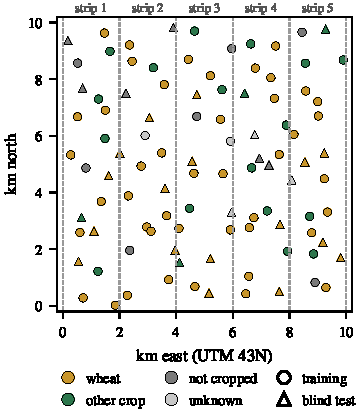
\includegraphics[width=0.48\linewidth]{figures/study_area.pdf}
  \caption{\todo{caption: what is plotted (points by class and role, the 5 strips) and what to notice}}
  \label{fig:area}
\end{figure}

% ---------------------------------------------------------------------------------------------
\section{Labels}
% This section is what makes the evaluation trustworthy: give it real space.
% [ ] Sampling: one random point per km$^2$ (seed 2026), so no one picks easy fields.
% [ ] Boundaries: grown from each point by NDVI similarity (threshold 0.08, calibrated by IoU on 3
%     known fields); 13 flagged outlines reviewed by eye (see README).
% [ ] Blind test set: 6 points per strip; labels from true-colour images only, never NDVI.
%     Be exact about who labelled what:
%       \NClaudeLabels{} labelled from true colour by an AI model (Claude), at the author's request;
%       \NNotFullyBlind{} of those after their NDVI had been seen during boundary review;
%       \NTestFromReview{} labelled non\_crop during boundary review, using imagery and NDVI.
% [ ] Training labels: k-means (k = 6) on the training fields' NDVI curves, clusters named from
%     their curves: \NCurveLabels{} labels. Note the circularity this creates (Discussion).
% [ ] Class merging (Table~\ref{tab:data}) and why: you cannot learn a class from 1 example.
% [ ] Figure~\ref{fig:profiles}: what separates the classes, in one or two sentences.
\todo{labels}

\begin{table}[t]
  \centering
  \caption{\todo{caption: the Rabi 2026 labels and how they were merged}}
  \label{tab:data}
  \begin{tabular}{llrr}
\toprule
Class used & Original label & Train & Test \\
\midrule
wheat & wheat & 44 & 17 \\
\midrule
other\_crop & other\_winter & 9 & 3 \\
 & short\_winter & 6 & 0 \\
 & sugarcane & 1 & 1 \\
 & orchard & 1 & 0 \\
\midrule
not\_cropped & non\_crop & 6 & 5 \\
 & fallow & 1 & 1 \\
\midrule
(left out) & unknown & 2 & 3 \\
\bottomrule
\end{tabular}

\end{table}

\begin{figure}[t]
  \centering
  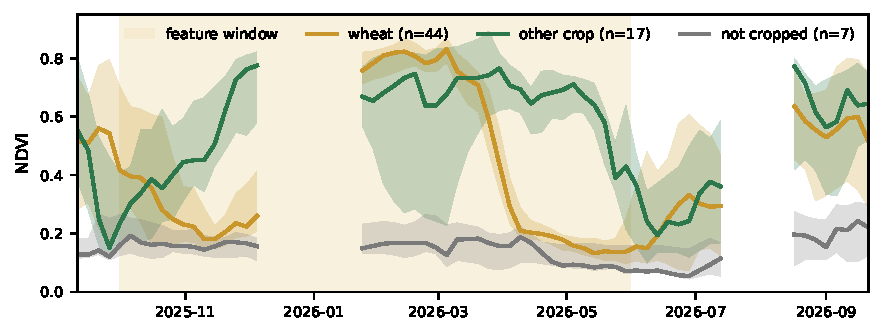
\includegraphics[width=\linewidth]{figures/profiles.pdf}
  \caption{\todo{caption: median and interquartile NDVI per class, training fields; what to notice}}
  \label{fig:profiles}
\end{figure}

% ---------------------------------------------------------------------------------------------
\section{Methods}
% [ ] Features. Set A: every index on every 5-day date from 1 Oct to 31 May, dates missing for
%     over half the fields dropped: \NFeatA{} features (5 x \NDatesA), more than the \NTrain{} fields.
%     Set B: \NFeatB{} hand-made features (list them briefly). Missing values: training-fold median.
% [ ] Models \cite{pedregosa2011sklearn}: majority baseline; L2 logistic regression, C in
%     {0.01, 0.1, 1, 10}; RBF SVM, C in {0.1, 1, 10, 100}; random forest \cite{breiman2001rf}, 500 trees;
%     gradient boosting \cite{friedman2001gbm}, 200 rounds of depth-2 trees, learning rate 0.05.
%     Balanced class weights. Write the regularised logistic loss as one equation.
% [ ] Evaluation:
%     - leave-one-strip-out CV, with C tuned inside the training strips only (nested)
%     - random stratified 5-fold CV, repeated 5 times, for comparison only \cite{roberts2017cv}
%     - selection: the simplest model within one standard error of the best \cite{hastie2009esl}
%     - the blind test set evaluated once, after the choice was fixed
% [ ] Metrics: accuracy, per-class recall, balanced accuracy (write its formula), and the
%     95\% interval $\pm 1.96\sqrt{p(1-p)/n}$.
\todo{methods}

% ---------------------------------------------------------------------------------------------
\section{Results}
% Facts only; meaning goes in Discussion.
% [ ] Table~\ref{tab:models}: \NNearTop{} models within one SE (\SE) of the best (\TopBal); the
%     chosen one: set \ChosenSet{} + \ChosenModel{}, C = \ChosenC.
% [ ] Spatial CV of the chosen model: \CVAcc{} accuracy (\CVCorrect/\NTrain), \CVBal{} balanced;
%     baseline \BaselineTrain. Random CV: \RandomBal{} balanced.
% [ ] Blind test (Table~\ref{tab:test}, Figure~\ref{fig:confusion}): \TestAcc{} (\TestCorrect/\NTest,
%     $\pm$\TestMargin{} points, so no lower than \TestLow), balanced \TestBal; baseline \BaselineTest{}
%     (\TestBaselineCorrect/\NTest). High-confidence test labels: \NHighCorrect/\NHigh.
% [ ] Label confidence: training on the \NTrainHighMed{} high/medium labels gave \ConfCleanAcc{}
%     (balanced \ConfCleanBal) vs \ConfAllAcc{} (\ConfAllBal) with all \NTrain.
% [ ] Figure~\ref{fig:weights}: which features carry the decision.
\todo{results}

\begin{table}[t]
  \centering
  \caption{\todo{caption: balanced accuracy (\%) by model, feature set and CV scheme; bold = chosen}}
  \label{tab:models}
  \begin{tabular}{lcccc}
\toprule
 & \multicolumn{2}{c}{Set A (200)} & \multicolumn{2}{c}{Set B (16)} \\
\cmidrule(lr){2-3}\cmidrule(lr){4-5}
Model & spatial & random & spatial & random \\
\midrule
Majority baseline & 33 & 33 & 33 & 33 \\
Logistic reg. & 98 & 97 & \textbf{98} & 96 \\
SVM (RBF) & 98 & 97 & 97 & 94 \\
Random forest & 92 & 95 & 98 & 97 \\
Gradient boosting & 98 & 91 & 98 & 98 \\
\bottomrule
\end{tabular}

\end{table}

\begin{table}[t]
  \centering
  \caption{\todo{caption: per-class recall of the chosen model, spatial CV vs blind test}}
  \label{tab:test}
  \begin{tabular}{lrrrr}
\toprule
 & \multicolumn{2}{c}{Spatial CV} & \multicolumn{2}{c}{Blind test} \\
\cmidrule(lr){2-3}\cmidrule(lr){4-5}
Class & $n$ & recall & $n$ & recall \\
\midrule
wheat & 44 & 44/44 & 17 & 17/17 \\
other\_crop & 17 & 16/17 & 4 & 3/4 \\
not\_cropped & 7 & 7/7 & 6 & 4/6 \\
\midrule
Accuracy & & 99\% & & 89\% \\
Balanced acc. & & 98\% & & 81\% \\
\bottomrule
\end{tabular}

\end{table}

\begin{figure}[t]
  \centering
  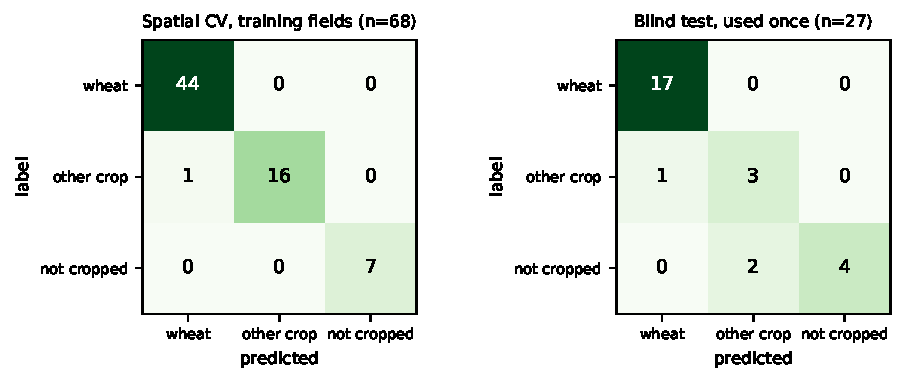
\includegraphics[width=0.85\linewidth]{figures/confusion.pdf}
  \caption{\todo{caption}}
  \label{fig:confusion}
\end{figure}

\begin{figure}[t]
  \centering
  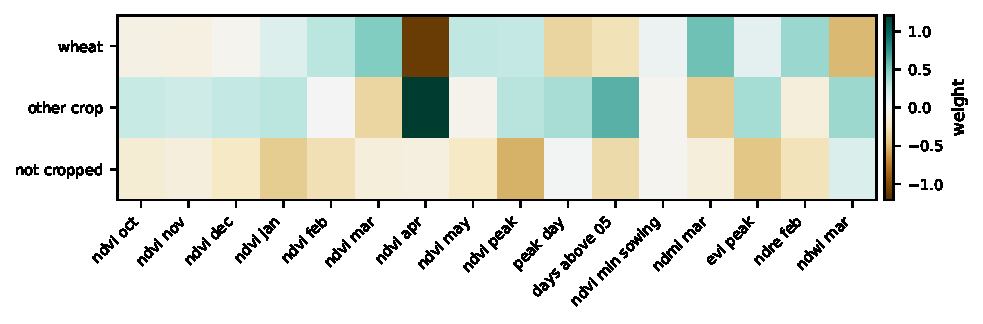
\includegraphics[width=\linewidth]{figures/weights.pdf}
  \caption{\todo{caption: logistic regression weights on standardised features, one row per class}}
  \label{fig:weights}
\end{figure}

% ---------------------------------------------------------------------------------------------
\section{Error analysis}
% One short paragraph per error, Figure~\ref{fig:errors}. For each: what the curve shows, why the
% model chose what it did, and whose error it really is (model, label, or boundary).
% [ ] g0000: canal-bank trees, labelled non_crop; green all winter. No green non-crop land in training.
% [ ] g0202: the point is on a road verge, the outline covers the green patch beside it.
% [ ] g0600: an early winter crop, harvested in early March, called wheat; the same confusion as the
%     only spatial-CV error (g0608, short_winter).
\todo{error analysis}

\begin{figure}[t]
  \centering
  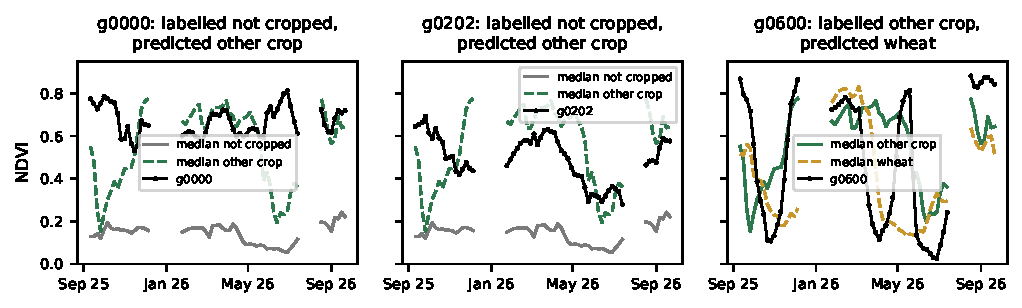
\includegraphics[width=\linewidth]{figures/errors.pdf}
  \caption{\todo{caption}}
  \label{fig:errors}
\end{figure}

% ---------------------------------------------------------------------------------------------
\section{Discussion and limitations}
% [ ] The main finding: the gap between CV and the blind test, and what explains it.
% [ ] Why set B matched set A, and why the simplest model was chosen.
% [ ] Why random vs spatial CV showed no gap here (ceiling), and why that does not show there is none.
% [ ] Limitations, named as the four threats from the lesson:
%     internal (circular training labels), construct (AI-read test labels; point vs outline),
%     external (one 10 x 10 km area, one year), statistical (\NTest{} test fields, $\pm$\TestMargin{} points).
% [ ] The test set has now been used: any change must be judged on new blind fields.
\todo{discussion}

% ---------------------------------------------------------------------------------------------
\section{Conclusion and future work}
% [ ] Two or three sentences restating the claim with its key numbers.
% [ ] Next steps you actually plan: Sentinel-1 radar for monsoon gaps, more and better labels
%     (a field visit), green non-crop examples, a second district.
\todo{conclusion}

% ---------------------------------------------------------------------------------------------
\section*{Reproducibility}
% [ ] Code and data: https://github.com/mburhankhan101-glitch/crop_project, commit \todo{hash}.
% [ ] Commands in order (README); seeds (2026 for sampling, 0 for models); Python 3.14.7,
%     scikit-learn 1.9.1.
\todo{reproducibility statement}

\section*{Use of AI tools}
% State plainly, in your words. Check your course's or venue's AI policy first.
% [ ] Code: written with an AI coding assistant (Claude Code), reviewed and run by you.
% [ ] Labels: \NClaudeLabels{} of the blind test labels were made by Claude from true-colour images,
%     at your request; \NNotFullyBlind{} of them were not fully blind. The training labels were proposed
%     from k-means clusters with Claude's help and reviewed.
% [ ] Writing: say what is yours (the text) and what help you had (outline, feedback).
\todo{AI use statement}

\section*{Acknowledgements}
Contains modified Copernicus Sentinel data (2025--2026), accessed through Microsoft Planetary Computer.

\bibliographystyle{plainnat}
\bibliography{references}

\end{document}
